
\chapter{Referencial teórico}

\section{Estado da arte}

A modelagem cinemática de robôs com cadeia fechada é uma área de grande relevância na robótica e tem sido objeto de intensa pesquisa nas últimas décadas, principalmente em trabalhos que investigam novas formas de aperfeiçoar o processo de calibragem desses manipuladores. Para calibrar um manipulador, diversas técnicas são utilizadas, mas inicialmente é necessário formular o modelo cinemático do equipamento o que é comum em diversos trabalhos.

Para o modelo cinemático de um manipulador robótico com a presença de geometria em paralelogramo e uma única cadeia fechada, como é o caso do modelo de robô ABB IRB 6660 (Fig. \ref{img:irb6660.jpg}), \citeauthoronline{peng2019} (\citeyear{peng2019}) utilizou a seguinte estratégia: abrir virtualmente essa cadeia, formando-se assim duas novas, a curta e a longa, que é o procedimento explicitado por \citeauthoronline{Siciliano2009} no seu livro Robotics modelling, planning and control (2.9.2). Ele cita outros trabalhos e como essa situação foi abordada, alguns pela cadeia curta e outros pela cadeia longa, chegando a conclusão de que a diferença entre os modelos cinemáticos não fica clara. Após a análise cinemática, fica evidente para o autor que os dois modelos alternativos possuem diferentes parâmetros, mas que por a cadeia curta ter uma estrutura mais simples, foi a cadeia adotada. Ao fim, o trabalho proposto teve maior eficiência computacional com praticamente a mesma precisão e é melhor para a calibragem cinemática em relação ao modelo baseado na cadeia longa.

\imagem{0.5}{irb6660.jpg}{ABB IRB 6660.}{ Adaptado de ABB Robotics}

Outra convenção usada foi na obtenção dos parâmetros de Denavit-Hartenberg (DH) para esse tipo de estrutura fechada. Os parâmetros de DH são obtidos de forma sequencial, frame a frame, mas é violado quando duas juntas consecutivas são paralelas, que é o caso de geometria em paralelogramo. Para contornar esse problema, \citeonline{hayati1983} propôs um modelo de DH modificado (MDH), com a introdução de um novo parâmetro rotacional em relação ao eixo y para descrever as juntas que fazem parte da cadeia fechada.

Essa abordagem foi utilizada por \citeauthoronline{towebb2012} (\citeyear{towebb2012}) no artigo An improved kinematic model for calibration of serial robots having closed-chain mechanisms (Um modelo cinemático aprimorado para calibração de robôs seriais com mecanismos de cadeia fechada em tradução livre) publicado por Cambrige University Press, juntamente com a abordagem citada anteriormente, abrindo  virtualmente a cadeia fechada. Levando em conta um manipulador Comau Smart H4 (Fig. \ref{img:smartH4.png}), esse trabalho propôs um método que melhorou a calibragem da precisão em comparação com o modelo cinemático curto (negligenciando  a estrutura em paralelogramo). Outros trabalhos também usaram a convenção de \citeonline{hayati1983}, como \citeonline{newman2000} e \citeonline{alici2005}.

\imagem{0.5}{smartH4.png}{Comau Smart H4.}{\cite{towebb2012}}

A modelagem da cinemática inversa de um manipulador robótico com três cadeias fechadas, como o EEZYbotARM, foi abordado pelo trabalho de \citeauthoronline{costa2017} (\citeyear{costa2017}). Utilizaram como modelo a ser estudado o protótipo MeArm v0.4, que assim como o EEZYbotARM é um projeto amador disponibilizado na plataforma Thingisverse e que se assemelha com o robô industrial ABB IRB 460 (Fig. \ref{img:figura13.jpg}). Uma consideração importante foi a posição da junta 3 ($\theta_3$), situada no ponto de rotação do elo 3. Porém a junta que ativamente faz esse movimento se localiza no elo 2, e que por meio de uma estrutura em paralelogramo, efetua o movimento do terceiro elo. Abordar o problema dessa maneira facilita o desenvolvimento do modelo geométrico desse manipulador. \citeonline{costa2017} então determinam as funções de junta que informam os valores de $\theta_1$, $\theta_2$ e $\theta_3$ em relação ao ponto (x, y, z).

\imagem{0.5}{figura13.jpg}{ABB IRB 460}{Fonte: ABB Robotics}

O trabalho de \citeauthoronline{gienke2019} (\citeyear{gienke2019}) busca prever e prevenir vibrações de acoplamento em manipuladores que executam usinagem. O modelo cinemático do manipulador ABB IRB 6660 foi feito levando em conta apenas a cadeia curta, pois apenas as juntas ativas e suas engrenagens poderiam causar vibrações, portanto as juntas passivas não foram modeladas.

\subsection{Trabalhos Relacionados ao CoppeliaSim}

O trabalho de  \citeauthoronline{wang2023} (\citeyear{wang2023}) utiliza o ambiente de simulação do CoppeliaSim para desenvolver redes neurais com conexões laterais, a fim de propor transferência externa de aprendizado de máquina para ajudar em novas tarefas. Novos métodos se mostraram eficazes em alcançar transferências de tarefas construindo conexões laterais entre redes neurais totalmente convolucionais, utilizando um modelo de braço robótico já presente no banco de dados do CoppeliaSim, o UR5, um braço robótico serial.

O estudo conduzido por \citeauthoronline{ferro2022} (\citeyear{ferro2022}) se concentra no desenvolvimento de simulações no ambiente CoppeliaSim para um manipulador robótico com geometria de paralelogramo que realiza procedimentos cirúrgicos minuciosos. A arquitetura em paralelogramo oferece a rigidez e precisão necessária para esse tipo de tarefa. Esse trabalho representa uma extensão do estudo anterior realizado por \citeauthoronline{fontanelli2018}  (\citeyear{fontanelli2018}), no qual a simulação cinemática do manipulador foi abordada. O estudo atual propõe estender a análise cinemática para incluir a simulação dinâmica do Kit de Pesquisas da Vinci, se valendo do poderio do CoppeliaSim para inserir informações que mais se aproximam da realidade, validando o sistema de controle desse manipulador, garantindo segurança nas atividades médicas.

\citeauthoronline{pereira} apresentam uma abordagem de simulação usando o CoppeliaSim e ROS (Robot Operating System) para demonstrar como os sensores a laser podem ser usados para localizar, identificar e pegar objetos e transportá-los para um local diferente. Em seu artigo, eles propõem algoritmos para permitir que um robô manipulador móvel navegue em seu ambiente e execute tarefas consideradas simples para humanos, mas complexas para robôs, como pegar pequenos objetos domésticos. O robô simulado consiste em uma base móvel acoplada a um manipulador Mico com seis graus de liberdade, e os algoritmos de controle incluem prevenção de colisões e reconhecimento de objetos. Os autores também discutem o potencial de aplicação dessa abordagem de simulação à robótica do mundo real.

\citeauthoronline{coelho2021}  (\citeyear{coelho2021}) apresentam um estudo sobre a locomoção de hexápodes em ambientes desafiadores usando o CoppeliaSim e o ROS. Sua pesquisa se concentra no uso de sensores de força para controlar as mudanças de fase da marcha de cada membro e se adaptar a novos pontos de apoio. Por meio de experimentos e simulações, eles avaliam a viabilidade desse sistema de controle e seu potencial para melhorar a autonomia dos hexápodes. Suas descobertas têm implicações importantes para o desenvolvimento de robôs hexápodes mais robustos e adaptáveis no futuro. De acordo com \citeauthoronline{coelho2021} (\citeyear{coelho2021}), o uso do CoppeliaSim e do ROS permite a avaliação não apenas do movimento gerado pelo hexápode, mas também do torque exigido pelos atuadores e das forças de interação. Esse software fornece uma estimativa das interações dinâmicas do sistema e pode estimar as possíveis falhas do hexápode durante a navegação. Além disso, ele fornece uma visão do comportamento dos controladores. Os autores observam que poucas pesquisas estudaram a locomoção de hexápodes nesse software, mas seu estudo demonstra seu potencial para avaliar a viabilidade dos controladores de hexápodes e melhorar sua autonomia em ambientes complexos.

\citeauthoronline{wang2022research} (\citeyear{wang2022research}) apresentam uma nova abordagem para o controle de braços robóticos móveis usando o aprendizado por reforço. O método proposto envolve o treinamento do braço robótico para executar uma tarefa específica, como abrir uma porta. Os pesquisadores usaram o CoppeliaSim para construir um ambiente de simulação para o braço robótico móvel e para treinar o algoritmo de aprendizagem por reforço. Isso permitiu que eles testassem a estratégia de controle em um ambiente seguro e controlado antes de aplicá-la a um cenário do mundo real. O controlador do manipulador foi feito em Python e os comandos enviados pela interface RemoteAPI do CoppeliaSim. Os resultados mostraram que o método proposto foi eficaz no controle do braço robótico e pode ser aplicado a uma variedade de cenários, incluindo resgate em ambientes perigosos e inspeção de equipamentos internos. 

 Através da conjunção do CoppeliaSim e do Robotics Toolbox for Python, este estudo busca estabelecer uma abordagem integrada e abrangente na simulação e análise de um braço robótico articulado com geometria em paralelogramo. Até o momento, observa-se uma lacuna na literatura científica quanto à exploração dessa configuração geométrica específica em um contexto simulado através do emprego destas ferramentas particulares.

\subsection{Simulador de Robô CoppeliaSim}

CoppeliaSim é uma ferramenta de simulação que permite aos usuários criar e testar sistemas robóticos virtuais. Possui uma interface amigável que permite aos usuários projetar e simular sistemas de vários robôs com facilidade. O software fornece uma ampla gama de modelos e componentes pré-construídos, tornando fácil para os usuários criar modelos robóticos personalizados. CoppeliaSim também pode simular o comportamento do robô em tempo real, tornando-o uma ferramenta ideal para testar e desenvolver algoritmos de controle \cite{nascimento2019}

O simulador CoppeliaSim se destaca como uma ferramenta amplamente utilizada para fins pedagógicos. Ele oferece um ambiente versátil e escalável para criar simulações em 3D em um curto espaço de tempo. Com sua arquitetura distribuída e baseada em scripts, cada objeto na cena pode ter um script embutido, permitindo operações simultâneas em forma de threads. Além disso, CoppeliaSim oferece diversos exemplos, modelos de robôs, sensores e atuadores para criar e interagir com um mundo virtual em tempo real \cite{Montenegro2022}.

 Diversos trabalhos têm utilizado a plataforma CoppeliaSim, abordando diferentes aplicações na robótica e sistemas multi-agente. Por exemplo, em \citeauthoronline{Obdrzalek2017} (\citeyear{Obdrzalek2017}) é apresentada uma estratégia para a utilização de um sistema multi-agente composto por Veículos Aéreos Não Tripulados (VANTs). Já \citeonline{knoll2017} propõe um esquema de navegação para robôs terrestres utilizando um conjunto de sensores de radiofrequência. Em \citeauthoronline{Tanberk2017} (\citeyear{Tanberk2017}) o simulador CoppeliaSim é empregado para testar um robô capaz de interpretar dados provenientes de um sensor Kinect, a fim de tomar decisões para a movimentação de peças em um jogo de xadrez. 

 O CoppeliaSim oferece uma interface de programação robusta e versátil, permitindo a criação de scripts personalizados para controle, análise e interação dos robôs e objetos no ambiente virtual. A ferramenta também suporta a integração de algoritmos de controle, proporcionando uma ampla gama de opções para experimentos e validações. A facilidade de uso do CoppeliaSim é destacada por sua interface gráfica intuitiva, que possibilita a configuração e visualização detalhada dos modelos robóticos e ambientes simulados. Além disso, o simulador oferece um extenso conjunto de recursos, como bibliotecas de modelos de robôs, sensores e atuadores, acelerando o processo de desenvolvimento de simulações. A possibilidade de comunicação em tempo real com as bibliotecas de programação mais populares, bem como com plataformas de hardware real, torna o CoppeliaSim uma escolha versátil para a validação e testes de algoritmos de controle em ambientes virtuais antes da implementação em robôs reais. Na versão mais recente, modulos de cinemática direta e inversa já vêm instalados. 

\subsection{Robotics Toolbox para Python}
O Robotics Toolbox para Python é uma biblioteca de funções e classes que fornece uma ampla gama de ferramentas para pesquisa e educação em robótica. Ele permite que os usuários criem e manipulem modelos robóticos, realizem análises cinemáticas e dinâmicas e simulem o comportamento do robô. \citeonline{haviland2023dkt1} propõem um tutorial em duas partes abordando a cinemática de robôs manipuladores, conceito fundamental no estudo e uso de braços robóticos. A caixa de ferramentas também fornece suporte para vários sensores e atuadores comumente usados em robótica, tornando possível criar simulações realistas e precisas de sistemas robóticos \cite{rtb2021}.

A biblioteca também disponibiliza recursos avançados para o planejamento de trajetórias, tornando possível simular e testar estratégias de movimentação em robôs móveis e manipuladores. Além disso, a integração do Robotics Toolbox for Python com outras bibliotecas populares de aprendizado de máquina e visão computacional permite o desenvolvimento de soluções mais abrangentes e inteligentes em aplicações de robótica \cite{rtb2021}. 

Quando usados em conjunto, CoppeliaSim e Robotics Toolbox para Python criam uma plataforma poderosa para simulação e modelagem de robótica. Os usuários podem projetar sistemas robóticos usando o Robotics Toolbox para Python e, em seguida, simular seu comportamento em CoppeliaSim. O Robotics Toolbox para Python também pode gerar as entradas necessárias para a simulação e analisar os dados de saída.


\section{Manipuladores Robóticos}

A globalização e abertura de mercado fomentou um aumento na produtividade, estimulando o lucro e a agilidade, e claro, reduzindo os custos. Para se manter competitivos, novas técnicas de produção foram pensadas ao longo das últimas décadas. Visando também uma uniformidade na produção e garantias na qualidade dos produtos, a indústria cada vez mais vem inserindo formas de automação e a utilização de robôs manipuladores, principalmente em tarefas pré-determinadas e repetitivas. Nesse cenário, manipuladores robóticos se mostram como a ferramenta ideal que propõe precisão e alta velocidade \cite{Vale2011}.

Um manipulador robótico é um dispositivo controlado por software, com uma
finalidade específica para os diversos tipos de processos automatizados. Muitas vezes se utilizam de sensores para auxiliar na movimentação e dar feedback ao controlador. Desde o primeiro manipulador patenteado por George Devol em 1954, mostrado na figura \ref{img:figura2.png}, até os dias de hoje, a robótica abraçou várias áreas do conhecimento como as engenharias mecânica, elétrica e da computação. Se desenvolveu impulsionada pela exploração subaquática e espacial, medicina e principalmente na indústria \cite{Lopes2002}.

\imagem{0.3}{figura2.png}{Unimate robot, por George Devol, 1961.}{\citeonline{IEEE2018}}

\subsection{Estrutura}

Atualmente muito utilizados nas indústrias, esses equipamentos são máquinas de grande investimento tecnológico. Geralmente são manipuladores do tipo antropomórficos, pois assemelham-se a um braço humano. Posicionados de forma fixa, possuem juntas flexíveis, braços e tronco. Na linguagem utilizada nesse trabalho, o tronco é a base do manipulador, geralmente dita como referencial do sistema e fixa no solo. Os braços são os elos (na literatura em inglês, links), conectados por juntas flexíveis (joints), e a última junta, o punho. O punho é responsável pela orientação final da extremidade do braço. Na extremidade então é fixada a ferramenta ou dispositivo o qual realiza a tarefa desejada. A ferramenta chamamos de órgão terminal. \cite{Spong2020}



\subsubsection{Juntas}

Segundo \cite{Santos2004} as juntas se dividem em tipos únicos para cada finalidade. Podem ser do tipo:
\begin{itemize}
	\item Prismática (P): essas movem-se em linha reta, compostas por duas hastes que
	deslizam entre si (Fig. \ref{img:subfigura1});
        
	\item Rotacional (R): as juntas rotacionais giram em torno de uma linha imaginária, o eixo
	de rotação (Fig. \ref{img:subfigura2}). Comumente, e nesse trabalho,
	estabelecemos que as juntas rotacionais giram em torno do eixo z;

	\item Esférica (S): as juntas esféricas funcionam como como uma combinação de três juntas
	rotacionais, tendo a liberdade de girar em torno dos três eixos, ilustrado \ref{img:subfigura3}.

	\item Cilíndrica ou Revolvente (V): basicamente composta por duas juntas, uma rotacional
	e outra prismática (Fig. \ref{img:subfigura4});

	\item Planar: formada por duas juntas prismáticas, permitindo movimentos em duas
	direções (Fig. \ref{img:subfigura5});

	\item Parafuso ou Torcional (T): é constituída por um parafuso e uma porca. Tem
	movimento semelhante ao da junta prismática, porém com movimento no eixo
	central, como ilustrado na figura \ref{img:subfigura6}.		\

\end{itemize}

\begin{figure}[!htb]
\centering
    \caption{\label{img:figura1} Tipos de Juntas}
    \subcaptionbox{\label{img:subfigura1} Junta prismática.}{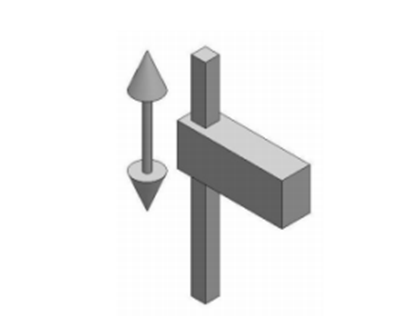
\includegraphics[scale=.55]{img/figura3.png}}
    \subcaptionbox{\label{img:subfigura2} Junta rotacional.}{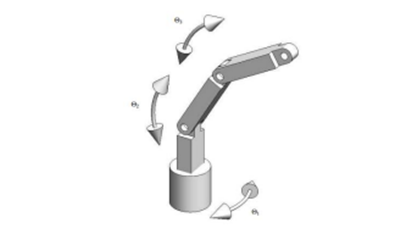
\includegraphics[scale=.55]{img/figura4.png}}
    \subcaptionbox{\label{img:subfigura3} Junta esférica.}{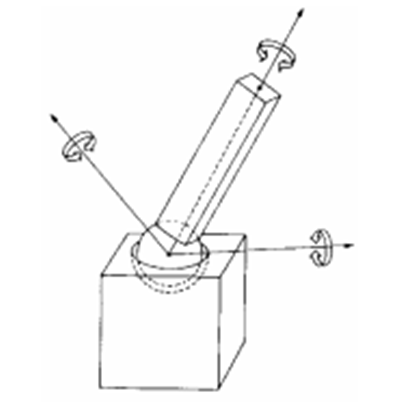
\includegraphics[scale=.55]{img/figura5.png}}
    \subcaptionbox{\label{img:subfigura4} Junta revolvente.}{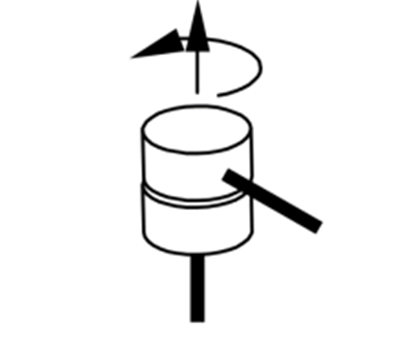
\includegraphics[scale=.55]{img/figura6.png}}
    \subcaptionbox{\label{img:subfigura5} Junta planar.}{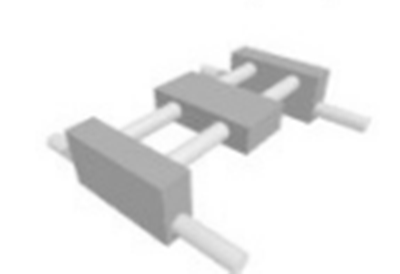
\includegraphics[scale=.55]{img/figura7.png}}
    \subcaptionbox{\label{img:subfigura6} Junta torcinal.}{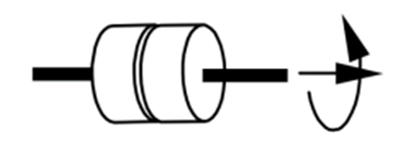
\includegraphics[scale=.55]{img/figura8.png}}
    \vspace{1.0em}
    \legend{\textbf{Fonte:} Adaptado de \citeonline{Santos2004}}
\label{fig:dag}
\end{figure}

As juntas do manipulador conferem diversos graus de liberdade - gdl - (Na literatura em inglês, Degrees of Freedom). E são os gdl que determinam os movimentos do manipulador no espaço tridimensional \cite{Santos2004}.

\subsubsection{Graus de Libertade (gdl) e graus de mobilidade (gdm)}

Os graus de liberdade definem o número total de movimentos independentes que o manipulador pode executar.

Diferentemente, os graus de mobilidade estão associados ao número de juntas existentes.

Um exemplo para demonstrar a diferença entre eles são os tripes, como esses usados por fotógrafos.  Em cada pé temos várias juntas prismáticas que permitem o movimento ao longo do mesmo eixo. Se em cada tripé houver três juntas, temos um tripé com 3 graus de liberdade mas 9 graus de mobilidade (3 gdl * 3 pés do tripé) \cite{Santos2004}.

\subsubsection{Tipos de configurações}

Como dito anteriormente, um manipulador robótico do tipo antropomórfico é formado por base, braço e órgão terminal. É a base que sustenta todo o manipulador, de onde o braço se movimenta, posicionando o punho no espaço. O punho então orienta o órgão terminal que por fim realiza sua função.

A configuração do manipulador é dada pelos tipos de juntas que ele possui. Então temos alguns tipos comuns de robôs manipuladores:

\begin{itemize}
	\item Manipulador cartesiano (PPP): é um manipulador composto por três juntas prismáticas - daí a representação das letras PPP. Consegue movimentar seu órgão terminal nas direções (x, y, z) do plano cartesiano. Na figura \ref{img:subfigura7} pode-se ver um exemplo de manipulador cartesiano, o robô Epson. Então as variáveis das juntas são coordenadas cartesianas do órgão terminal em relação a base.		\

	\item Manipulador Cilíndrico (RPP): o manipulador cilíndrico é formado por uma primeira junta rotacional na base e a segunda e terceira juntas são prismáticas, recebendo esse nome porque as variáveis das juntas são as coordenadas cilíndricas do órgão terminal em relação a base. Na figura \ref{img:subfigura8} é exemplificado o robô cilíndrico Seiko RT3300.

	\item Manipulador Esférico (RRP): formado pela primeira junta rotacional em relação a
	base, a segunda também rotacional e a terceira junta prismática. Todas as três juntas
	são dispostas de modo que seus eixos de trabalho são perpendiculares entre si. O
	termo manipulador esférico se justifica porque coordenadas esféricas definem a
	posição do órgão terminal em relação à origem. A origem nesse caso não é na base,
	mas na intersecção dos três eixos z (eixo o qual a junta rotaciona em torno). Na figura
	\ref{img:subfigura9} temos o Stanford Arm, um dos mais conhecidos robôs esféricos.
		
	\item Manipulador SCARA (RRP): : O acrônimo SCARA se traduz como Robô Articulado
	Seletivo Compatível para Montagem (Selective Compliant Articulated Robot for
	Assembly), exemplificado na figura \ref{img:subfigura10}. É um manipulador bastante popular, e como o
	nome sugere, ideal para operações de montagem, e se difere em relação ao manipulador
	esférico na orientação dos eixos z das juntas. Aqui os três eixos $z_1$, $z_2$ e $z_3$ são
	paralelos entre si.

	\item Manipulador Articulado (RRR): é o manipulador chamado também de
	antropomórfico ou manipulador de revolução. Nele é muito usada uma configuração
	de ligação em paralelogramo. Nesse arranjo temos três juntas rotacionais. A segunda e
	terceira juntas possuem seus eixos de rotação $z_2$ e $z_3$ paralelos entre si. E $z_2$ e $z_3$ são
	perpendiculares ao eixo de rotação $z_1$ da primeira junta. Na figura \ref{img:subfigura11} observa-se o robô
	articulado ABB IRB 460, que possui uma grande área de movimento e se mantém
	compacto. Esse arranjo de ligação em paralelogramo possui algumas vantagens, como
	o fato de que o atuador da terceira junta poder ficar localizado no primeiro elo. Dessa
	forma, o peso do motor fica no primeiro elo, e o segundo e terceiro elo ficam mais
	leves, sobrando mais potencia para realizar a tarefa em si. Por isso são muito usados em operações com carga útil pesada \cite{Siciliano2009}. E ainda, esse arranjo é
	mais simples de se analisar sua dinâmica, que se traduz em vantagem para etapas de planejamento de trajetória e o desenvolvimento do controlador \cite{Spong2020}.
	
\end{itemize}

\subsubsection{Braços robóticos com geometria do paralelogramo}
.

Uma das configurações dos manipuladores robóticos é do tipo paralelo. Diferente da configuração serial, a configuração do tipo paralelo possui duas ou mais cadeias cinemáticas fechadas, ligando a base ao órgão efetuador na ponta \cite{Siciliano2009}. Esse tipo de configuração garante mais firmeza e rigidez, dessa forma sendo mais preciso que configurações de cadeia aberta.

Manipuladores antropomórficos, como o braço robótico, mais especificamente do tipo “cotovelo ", possuem também cadeias cinemáticas fechadas em geometrias de paralelogramo. Além da rigidez, esse tipo de configuração também reduz a quantidade de espaço necessário para o braço. Isso porque a geometria em paralelogramo permite que o braço se estenda verticalmente, sem exigir espaço adicional horizontalmente.

Braços robóticos com geometria de paralelogramo são frequentemente utilizados em tarefas de montagem e tarefas do tipo \textit{pick and place}, como posicionar produtos em caixas ou paletes (paletização). Da mesma forma, são utilizados em tarefas de pintura e soldagem. Por sua capacidade de alta precisão, também são utilizados em procedimentos médicos, como posicionar instrumentos cirúrgicos com precisão e delicadeza.
\begin{figure}[!htbp]
\centering
    \caption{\label{img:figura2} Configurações do manipulador}
    \subcaptionbox{\label{img:subfigura7} Robô cartesiano da Epson.}{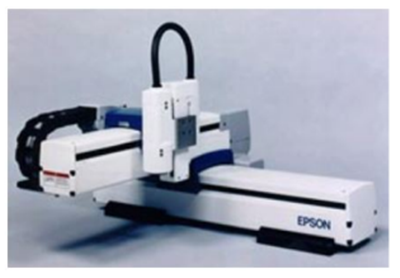
\includegraphics[scale=.6]{img/figura9.png}}
    \subcaptionbox{\label{img:subfigura8} Robô cilíndrico Seiko RT3300.}{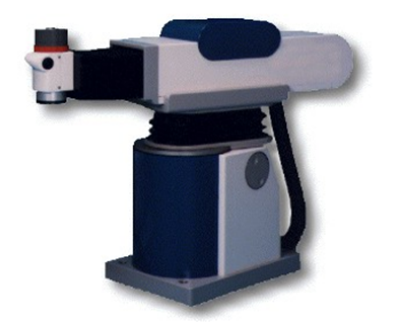
\includegraphics[scale=.6]{img/figura10.png}}
    \subcaptionbox{\label{img:subfigura9} Stanford Arm, manipulador esférico.}{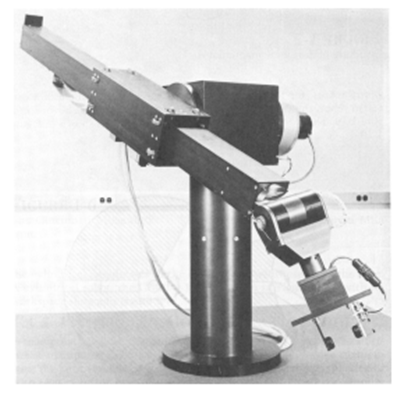
\includegraphics[scale=.6]{img/figura11.png}}
    \subcaptionbox{\label{img:subfigura10} Robô SCARA Epson E2L653S.}{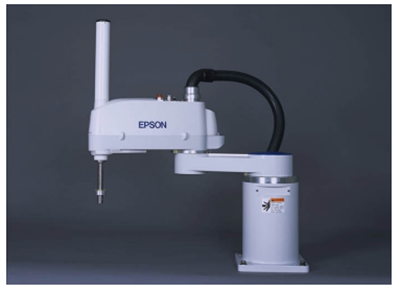
\includegraphics[scale=.6]{img/figura12.png}}
    \subcaptionbox{\label{img:subfigura11} Robô articulado com geometria em paralelogramo ABB IRB 460.}{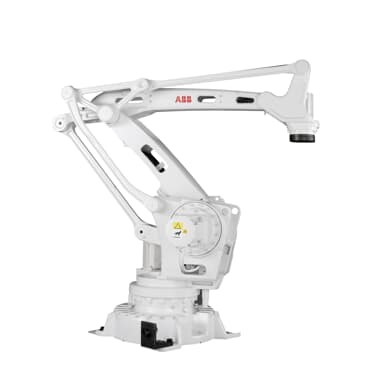
\includegraphics[scale=.6]{img/figura13.jpg}}
    \vspace{1.5em}
    \legend{\textbf{Fonte:} \citeonline{Spong2020}}
\label{fig:dag}
\end{figure}
\pagebreak

\subsection{Cinemática Direta}

Esses elos ligados por juntas então formam uma cadeia cinemática. Imagine um cenário onde queremos fazer o órgão terminal sair da posição inicial home, ir até um ponto A no espaço, percorrer um caminho S até chegar ao ponto B. São vários problemas a serem resolvidos a fim de conseguir executar tal ação.

A cinemática direta descreve a posição do órgão terminal (x, y, z) com base nos parâmetros dos ângulos das juntas que formam o braço robótico $\theta_1, \theta_2, \theta_3$. Dessa forma, a posição e orientação do órgão terminal pode ser expressa por uma função das variáveis conjuntas. Comumente o manipulador consegue informar sua posição com base nos ângulos das juntas por meio de sensores (encoders nos servo-motores que indicam sua angulação).

Para fazer a modelagem da cinemática direta utiliza-se o método de Denavit-Hartenberg (DH)  para obtenção dos parâmetros envolvidos. Os parâmetros de DH fazem parte de uma convenção popular, introduzida em 1955, na qual uma matriz de transformação homogênea é descrita por meio de quatro parâmetros, e que leva as coordenadas do $frame_i$ para o $frame_i+1$ \cite{Spong2020}.

\subsubsection{Convenção de Denavit-Hartenberg}

Sendo um manipulador formado por um conjunto de elos conectados por juntas formando uma cadeia cinemática, é necessário definir a identificação de cada componente. Os elos, então, são numerados a partir da base, sendo o primeiro o elo 0. Quanto às juntas, a primeira é a número 1. Dessa forma, em qualquer configuração do manipulador, a junta $i$ conecta os dois elos, $i-1$ e $i$ \citeonline{Spong2020}.

O método de DH consiste em três etapas principais: definir os sistemas de coordenadas, definir os parâmetros e então construir a matriz de transformação homogênea.

\begin{enumerate}
	\item Sistema de coordenadas: As escolhas de sistema de coordenadas podem variar, porém todas elas chegam ao mesmo resultado para uma dada estrutura. Aqui usaremos o eixo $z_i$ ao longo do eixo da junta $i+1$, como mostra a ilustração \ref{img:figura14.png}.
	\item Definição dos Parâmetros: A figura \ref{img:figura14.png} exemplifica dois elos conectados por uma junta. Daí obtém-se os quatro parâmetros para a convenção DH dessa junta e os dois elos, definindo o comportamento dos desses. São eles:
	
		\begin{itemize}
			\item $a_i = tamanho\:do\:elo;$
			\item $d_i = deslocamento\:do\:elo;$
			\item $\alpha_i = giro\:do\:elo;$
			\item $\theta_i =  \hat{a}ngulo\:da\:junta. $
		\end{itemize}
	
	\imagem{.5}{figura14.png}{Parâmetros de Denavit-Hartenberg.}{\citeonline{Siciliano2009}}
	
	\item  Matriz de Transformação Homogênea: Com os parâmetros definidos, a última etapa é montar a matriz de transformação homogênea. Dos quatro parâmetros, dois estão associados à componente móvel, às juntas. Se a junta for prismática, a variável da junta é o deslocamento di. Se for uma junta rotacional, a variável em questão será $\theta_i$. Os outros dois parâmetros estão associados aos elos, são fixos. A matriz de transformação homogênea é dada por \eqref{eq:1}:

\begin{equation}
	A_i = Rot(z,\theta_1)Trans(a_i, 0, 0)Trans(0, 0, d_i)Rot(x,\alpha_i)
	\label{eq:1}
\end{equation}
		
e a transformação que descreve a cinemática da base em relação ao punho (último frame antes do órgão terminal) é dado por \eqref{eq:2}:

\begin{equation}
	^0T_n = A_0A_1...A_n
	\label{eq:2}
\end{equation}

\end{enumerate}

\subsection{Cinemática Inversa}
A análise da cinemática inversa nos fornece as funções que relacionam a posição Pw do punho (x, y, z), frame o que se posiciona o órgão terminal, com os valores das juntas ($\theta_i$). Pode-se dizer que são
exatamente o inverso das funções que a cinemática direta nos fornece. Simbolicamente dado por \eqref{eq:3},

\begin{align}
	&\vec{r} = \vec{F}(q); \nonumber\\
	&q = \vec{F}^{-1}\vec{(r)}; \vec{F}^{-1} :\Re^n \rightarrow \Re^6
	\label{eq:3}
\end{align}

Graficamente, entende-se como ilustrado em \ref{img:figura15.png}:

	\imagem{1.0}{figura15.png}{Relação entre cinemática inversa e direta.}{ Adaptado de \citeonline{Santos2004}}

Muitas vezes, o problema da cinemática inversa não tem solução. Ou ainda, pode assumir infinitas soluções. Resolver esse problema analiticamente muitas vezes se
mostra uma tarefa onerosa. Alternativamente, adotar métodos numéricos iterativos, mesmo
que sejam menos precisos, pode ser melhor se a cada iteração o método convergir para o
desejado, com base em valores sugeridos para as variáveis.

Métodos como esse utilizam a matriz jacobiana do manipulador. O jacobiano J é
composto pelas derivadas parciais das posições do órgão terminal em relação aos ângulos
das juntas, dado em \eqref{eq:4}. Portanto, dado um deslocamento infinitesimal, o jacobiano expressa a relação entre o deslocamento das juntas e a localização do órgão terminal. Em outras palavras, ao
invés de descrever a posição do órgão terminal, o jacobiano descreve seu movimento\cite{Nilsson2009}.

\begin{equation}
J = \begin{vmatrix}
		\displaystyle
			\frac{\delta x_e}{\theta_1} & \displaystyle ...  & \displaystyle \frac{\delta x_e}{\theta_n} \\ 
		\displaystyle
			\frac{\delta y_e}{\theta_1} & \displaystyle ...  & \displaystyle \frac{\delta y_e}{\theta_n} \\ 
		\displaystyle
			\frac{\delta z_e}{\theta_1} & \displaystyle ...  & \displaystyle \frac{\delta z_e}{\theta_n} \\ 
	\end{vmatrix} 
	\label{eq:4}
\end{equation}

\citeonline{Craig2005} descreve o jacobiano como sendo derivadas multidimensionais. Se temos seis funções, por exemplo, cada uma delas sendo funções de seis variáveis independentes, como mostra \eqref{eq:7}

\begin{align}
	&y_1 = f_1(x_1,x_2,x_3, x_4, x_5, x_6), \nonumber\\
	&y_2 = f_2(x_1,x_2,x_3, x_4, x_5, x_6), \nonumber\\
	&\vdots \nonumber\\
	&y_6 = f_6(x_1,x_2,x_3, x_4, x_5, x_6),
	\label{eq:7}
\end{align}

Se usarmos a notação de vetores, teríamos \eqref{eq:8}

\begin{equation}
	Y = F(X)
	\label{eq:8}
\end{equation}

E se queremos calcular a derivadas de $y_1$ em função das variáveis $x_j$, usando a regra da cadeia, teremos \eqref{eq:9}

\begin{align}
	&\delta y_1 = \frac{\partial f_1}{\partial x_1} \delta x_1 + \frac{\partial f_1}{\partial x_2} \delta x_2 + \ldots + \frac{\partial f_1}{\partial x_6} \delta x_6, \nonumber\\
	&\delta y_2 = \frac{\partial f_2}{\partial x_1} \delta x_1 + \frac{\partial f_2}{\partial x_2} \delta x_2 + \ldots + \frac{\partial f_2}{\partial x_6} \delta x_6, \nonumber\\
	&\vdots \nonumber\\
	&\delta y_3 = \frac{\partial f_3}{\partial x_1} \delta x_1 + \frac{\partial f_3}{\partial x_2} \delta x_2 + \ldots + \frac{\partial f_3}{\partial x_6} \delta x_6,
	\label{eq:9}
\end{align}

Novamente, podemos escrever de uma forma mais simples, usando a notação vetorial \eqref{eq:10}

\begin{equation}
	\delta Y = \frac{\partial F}{\partial X} \delta X.
	\label{eq:10}
\end{equation}

E essa matriz $6x6$ de derivadas parciais em \eqref{eq:10} que chamamos de Jacobiano, J. Como as funções $f_1(x)$ até $f_6(x)$ são não-lineares, podemos usar a notação \eqref{eq:11} \cite{Craig2005}:
\begin{equation}
	\label{eq:11}
	\delta Y = J(X)\delta X.
\end{equation}

Então, para resolver o problema da cinemática inversa por métodos numéricos
iterativos, podemos usar o método dos mínimos quadrados. Basicamente, esse método busca
reduzir a soma dos quadrados das diferenças entre o valor proposto e o valor real da posição
do órgão terminal, onde as variáveis são os ângulos das juntas. Existem também outros métodos e ferramentas de modelagem, como o Robotics Toolbox for Python, por Peter Corke. Esse Toolbox possui métodos e funções para lidar com matrizes de transformação, jacobianos e controle de modelos de robôs dos mais diversos tipos \cite{rtb2021}, e inclui a solução de cinemática inversa por meio dos métodos de Newton-Raphson (NR),  Gauss-Newton (GN) e Levenberg-Marquardt (LM).

\citeonline{Craig2005} indica que na robótica geralmente se usa o jacobiano para relacionar as velocidades das juntas com velocidades cartesianas do punho do braço robótico, por exemplo \eqref{eq:12}
\begin{equation}
	^0v = ^0J(\Theta)\dot{\Theta}
	\label{eq:12}
\end{equation}
Onde $\Theta$ é o vetor de ângulos das juntas do manipulador, e $v$ é o vetor de velocidades cartesianas. Esse vetor de velocidades cartesianas é formado pelo vetor de velocidades lineares com o vetor de velocidade rotacional, como mostra \eqref{eq:13}
\begin{equation}
	\displaystyle ^0v = \begin{bmatrix}
		\displaystyle ^0 \upsilon \\
		\displaystyle ^0 \omega 
	\end{bmatrix}
	\label{eq:13}
\end{equation}

É importante salientar ainda que, dado um jacobiano descrito para um frame $\left \{ B \right \}$, isso é
\begin{equation}
	\begin{bmatrix}
		\displaystyle ^B \upsilon \\
		\displaystyle ^B \omega 
	\end{bmatrix} = ^B v = ^B J(\Theta)(\dot\Theta)
	\label{eq:15}
\end{equation}

podemos expressar esse Jacobiano em outro frame $\left \{ A \right \}$ pela transformada dada em \eqref{eq:14}:
\begin{equation}
	\begin{bmatrix}
		\displaystyle ^A \upsilon \\
		\displaystyle ^A \omega \\
	\end{bmatrix} = \begin{bmatrix}
		^A_BR  &  0\\ 
		0 &  ^A_BR
		\end{bmatrix} \begin{bmatrix}
		\displaystyle ^B \upsilon \\
		\displaystyle ^B \omega \\
	\end{bmatrix}
	\label{eq:14}
\end{equation}

E, dado \eqref{eq:15}, fica claro que para mudar o frame de referência do jacobiano usamos a relação \eqref{eq:16} \cite{Craig2005}:
\begin{equation}
	^A J(\Theta) = \begin{bmatrix}
		^A_BR  &  0\\ 
		0 &  ^A_BR
		\end{bmatrix} {^BJ(\Theta)}.
		\label{eq:16}
\end{equation}

\citeonline{Craig2005} afirma ainda que, se a matriz jacobiana não for singular, poderemos invertê-la para obter os ângulos das juntas dada as velocidades cartesianas, da forma de \eqref{eq:17}:
\begin{equation}
	\dot\Theta = J^{-1}(\Theta) \upsilon.
	\label{eq:17}
\end{equation}

Porém, na maioria dos manipuladores, os valores de $\Theta$ podem produzir um jacobiano singular. Esses valores costumam ser ou nos limites do espaço de trabalho do manipulador, ou mesmo dentro do volume do espaço de trabalho. Essas posições de singularidade indicam posições impossíveis de alcançar, a a inversa do jacobiano tende ao infinito \cite{Craig2005}.
%Se multiplicarmos a matriz jacobiana do manipulador pelo vetor da variação
%infinitesimal das posições das juntas $\Delta \theta $, teremos $\Delta P$, a mudança na posição do órgão %terminal, determinado por \eqref{eq:5}.
%\begin{equation}
%	\Delta P = J(\theta )\Delta (\theta )
%	\label{eq:5}
%\end{equation}
%
%Essa equação se assemelha ao problema da cinemática direta. Tratando do problema
%da cinemática inversa, podemos encontrar $\Delta \theta $ invertendo a matriz jacobiana $J(\theta)$. Teremos %\eqref{eq:6}:
%
%\begin{equation}
%	\Delta \theta = J(\theta )^{-1} \Delta P
%	\label{eq:6}
%\end{equation}
%
%Como o jacobiano é calculado por meio de aproximações lineares, o resultado da
%equação também é uma aproximação da variação dos ângulos das juntas. Devido a isso, um
%método iterativo se adequa, pois as variações são calculadas repetidamente \cite{Nilsson2009}.

O objetivo do trabalho já citado de \cite{costa2017} é a modelagem da cinemática inversa do protótipo MeArm v0.4. De forma resumida os resultados foram obtidos pelo método geométrico, avaliando os ângulos das juntas ativas $(\theta_1,\theta_2, \theta_3)$  em relação com a posição $(x, y, z)$ do efetuador por meio de relações trigonométricas e lei dos cossenos (Fig. \ref{img:eezybootarm-mk2-kinematic-points.jpg}).  Para o angulo $\theta_1$, que posiciona o efetuador final no plano $xy$ \eqref{eq:19}:

\imagem{0.5}{eezybootarm-mk2-kinematic-points.jpg}{Aplicação da lei dos cossenos}{Adaptado de: José (2020)}

\begin{equation}
	\theta_1 = \arctan \left (\frac{p_y}{p_x}\right ) = arctan \left ( \frac{y}{x} \right )
	\label{eq:19}
\end{equation}

Para os ângulos $\theta_2$ e $\theta_3$ o resultado do artigo foi \eqref{eq:20} e \eqref{eq:21}:
\begin{equation}
    \theta_2 = arctan \left (\frac{p_z - d_2}{p_x}\right ) - arctan\left (\frac {a_3\sin\theta_3 }{a_2 + a_3\cos\theta_3}\right ) 
    \label{eq:20}
\end{equation}
\begin{equation}
    \theta_3 = \arccos \left ( \frac{(p_x - a_1 - f\cos\theta_1)^2 + (p_z-d_2)^2 - a_2^2-a_3^2}{2a_2a_3} \right )
    \label{eq:21}
\end{equation}
sendo $px$, $pz$ e $py$ os pontos cartesianos no espaço desejados para o órgão efetuador final, $a_1$, $a_2$ e $a_3$ sãos as dimensões dos braços do EEzybotArm. Nas equações \eqref{eq:20} e \eqref{eq:21}, $p_z - d_2$ refere-se ao valor de $z_1$, que é a distancia entre a junta $\#1$ e a junta $\#4$.